Cross-stitch is a form of needlework known since prehistoric times. A cross-stitch pattern consists of several crosses on the face of the fabric, that are connected on the backside. Traditionally, the whole pattern should be embroidered by one thread.

Carol is going to mass-produce cross-stitch patterns. Each pattern will be accompanied by the rectangular patch of fabric and the thread that is required to embroider this pattern. Carol wants to minimize the length of the thread that is required for the pattern.\\
\centerline{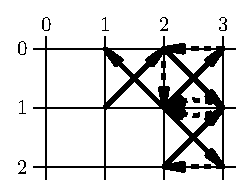
\includegraphics{cross-stitch-1.ps}}\\
You are given the face of the pattern. You should design the backside, so that the total length of the thread is minimal. The crosses on the pattern's face are 8-connected, i.e. it is possible to reach each cross from any other by a sequence of chess king's moves.